\documentclass[9pt]{IEEEtran}

\usepackage[english]{babel}
\usepackage{booktabs}
\usepackage{graphicx}
\usepackage[utf8]{inputenc}
\usepackage[T1]{fontenc}
\usepackage{lmodern}
\input{glyphtounicode}
\pdfgentounicode=1

\title{\vspace{0ex}Exercise 2: Mean-Shift Tracking}
\author{Dino D\v{z}aferagi\'c\vspace{-4.0ex}}

\begin{document}
\maketitle

\section{Introduction}
This project has two core tasks.
The first task is mean-shift mode seeking on response maps.
The second task is a color-based mean-shift tracker.
I implemented both tasks in Python and tested them on the required data.
I then ran extra and bonus experiments from the grading section.

\section{Experiments}
This section follows the grading tasks.

\subsection{Mean-shift mode seeking}
I tested two kernels (Epanechnikov, Gaussian), three bandwidths (11, 21, 31), three stop criteria (1.0, 0.5, 0.1), and four start points.
Table~\ref{tab:mode_seeking} shows the main pattern from the runs.
Figure~\ref{fig:ms_paths} shows convergence trajectories on the provided response map.

\begin{figure}[h]
    \centering
    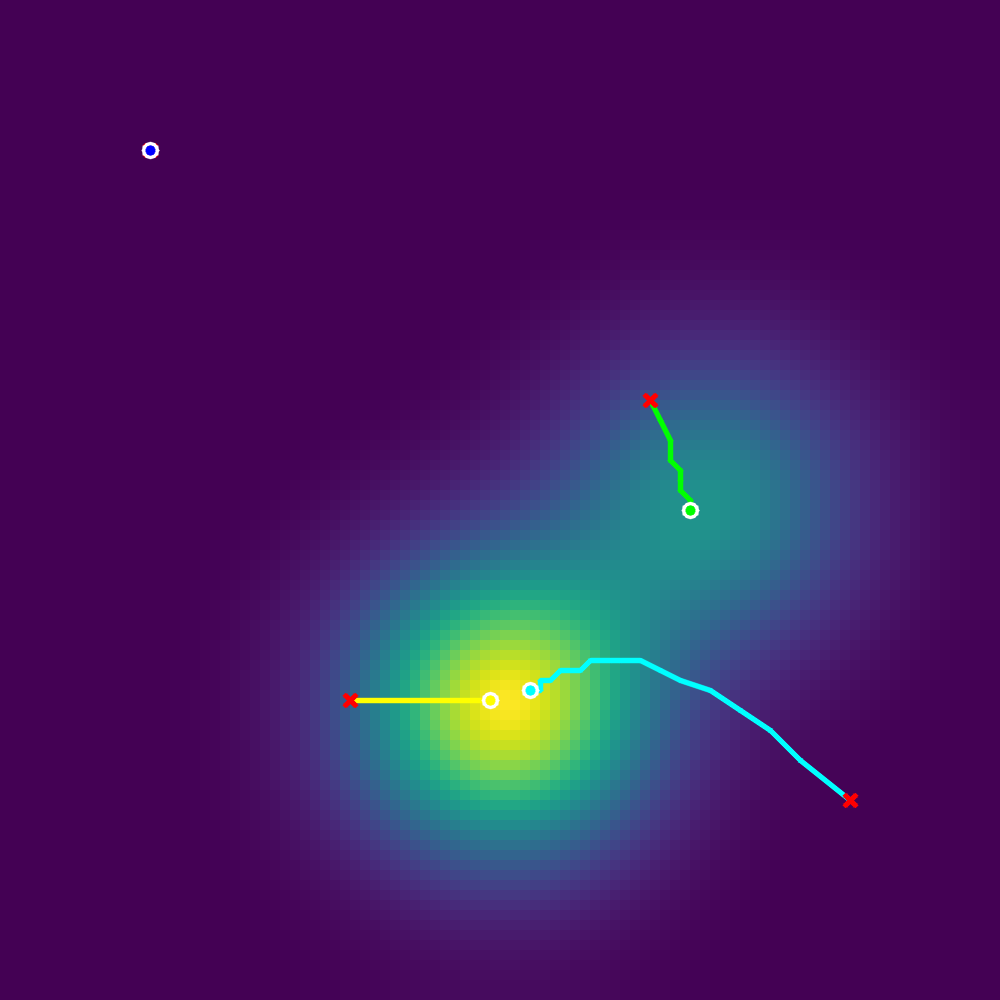
\includegraphics[width=0.92\linewidth]{ms-material/mode_seeking_paths_provided_clean.png}
    \caption{Mean-shift convergence trajectories on the provided response map. Red marks show start points. Colored lines show iterative paths.}
    \label{fig:ms_paths}
\end{figure}

\begin{table}[h]
    \centering
    \caption{Mode-seeking behavior summary}
    \label{tab:mode_seeking}
    \begin{tabular}{llll}
        \toprule
        Kernel       & Bandwidth & Stop eps & Typical result       \\
        \midrule
        Epanechnikov & 11        & 1.0      & fast, local moves    \\
        Epanechnikov & 21        & 0.5      & stable tradeoff      \\
        Epanechnikov & 31        & 0.1      & often hits 100 steps \\
        Gaussian     & 11        & 0.5      & moderate speed       \\
        Gaussian     & 21        & 0.1      & many long runs       \\
        Gaussian     & 31        & 0.5      & stable global pull   \\
        \bottomrule
    \end{tabular}
\end{table}

The start point has strong effect.
When the start is far from a strong peak, the method can stall or move slowly.
A strict stop threshold (0.1) often increases steps a lot.
In my setup, bandwidth 21 with stop threshold 0.5 gave a good balance.

\subsection{Tracker on five sequences}
I evaluated the tracker on five VOT2014 sequences: \texttt{polarbear}, \texttt{hand1}, \texttt{fernando}, \texttt{drunk}, \texttt{basketball}.
I count a tracking failure when overlap is 0 or less; after each failure, the evaluation skips 5 frames and then reinitializes the tracker.
Table~\ref{tab:required_tracker} gives the required results.

\begin{table}[h]
    \centering
    \caption{Required tracker results (5 sequences)}
    \label{tab:required_tracker}
    \begin{tabular}{lcc}
        \toprule
        Sequence    & FPS   & Failures \\
        \midrule
        polarbear   & 381.0 & 0        \\
        hand1       & 289.6 & 4        \\
        fernando    & 87.1  & 1        \\
        drunk       & 169.7 & 0        \\
        basketball  & 224.2 & 1        \\
        \midrule
        Total / Avg & 230.3 & 6        \\
        \bottomrule
    \end{tabular}
\end{table}

\subsection{Own function for mode seeking}
I added a custom response landscape with three peaks in \texttt{run\_mode\_seeking.py}.
The method converged on this map and showed the same behavior trends as on the provided map.
This confirms that the implementation is not tied to one specific response shape.
From the script output, the provided map had \texttt{avg steps=23.00}, \texttt{min=0}, \texttt{max=100}, while the custom map had \texttt{avg steps=8.26}, \texttt{min=3}, \texttt{max=29}.
This shows that the custom landscape was easier for convergence than the provided one.

\subsection{Failure case analysis}
The hardest case was \texttt{hand1} with 4 failures.
In good frames, the box is centered on the raised hand.
In bad frames, fast hand motion and blur push the box toward wrist or nearby background.

In \texttt{drunk}, the target is a dark car in a street scene with other similar cars.
Good frames show the box on the target car.
Bad frames are suspicious when the box shifts to another car region with similar color and shape.

In \texttt{fernando}, the scene contains two cats in an indoor environment.
Good frames lock on the intended cat.
Suspicious frames appear when the cats cross and the box may switch identity for a short time.

In \texttt{basketball}, the target player in green is tracked well in many frames.
In bad frames, the box can move to another nearby player with similar jersey color.

In \texttt{polarbear}, the tracker is stable over the full sequence (0 failures).
Some frames are still suspicious because white target regions are similar to snow, but no official failure occurred.

Main improvement idea: combine color cues with an extra feature (for example gradient or texture) and use stronger motion prediction during fast changes.

\subsection{Parameter impact}
I tested bins, kernel size, stop criterion / iterations, and update speed.
Table~\ref{tab:param_impact} summarizes total failures and average FPS on the same five sequences.
For backprojection weights, I used \(v = q / (p + \epsilon)\) (without square root). The slide form with \(\sqrt{q/(p+\epsilon)}\) is also valid, but this simpler ratio gave stable behavior in this implementation and parameter setup.

\begin{table}[h]
    \centering
    \caption{Parameter impact summary}
    \label{tab:param_impact}
    \begin{tabular}{lcc}
        \toprule
        Setting                            & Total failures & Avg FPS           \\
        \midrule
        \texttt{nbins=8/16/32}             & 9/6/10         & 408.1/255.3/107.2 \\
        \texttt{window\_scale=1.5/2.0/2.5} & 6/6/6          & 208.5/295.2/259.3 \\
        \texttt{kernel\_sigma=0.8/1.0/1.2} & 27/6/8         & 104.4/275.1/502.5 \\
        \texttt{stop\_eps=1.0/0.5/0.2}     & 9/6/8          & 453.4/278.7/122.5 \\
        \texttt{max\_iters=10/20/35}       & 7/6/6          & 348.8/285.9/219.7 \\
        \texttt{model\_alpha=0.0/0.05/0.2} & 5/6/7          & 294.9/285.7/274.0 \\
        \bottomrule
    \end{tabular}
\end{table}

High bin count increased cost and did not help in this setup.
Kernel settings mattered a lot; poor kernel scale (\texttt{kernel\_sigma=0.8}) gave many failures.
Very loose stopping (\texttt{stop\_eps=1.0}) was fast but less robust.
In this subset, no model update (\texttt{model\_alpha=0.0}) gave the lowest failure count.

\subsection{Color spaces and background model}
I tested four color spaces.
I also added background histogram modeling.
Table~\ref{tab:bonus} shows the result.

\begin{table}[h]
    \centering
    \caption{Bonus experiments}
    \label{tab:bonus}
    \begin{tabular}{lcc}
        \toprule
        Experiment                     & Total failures & Avg FPS \\
        \midrule
        \texttt{BGR}                   & 6              & 276.1   \\
        \texttt{HSV}                   & 10             & 159.2   \\
        \texttt{Lab}                   & 7              & 233.5   \\
        \texttt{YCrCb}                 & 9              & 258.3   \\
        \texttt{no background model}   & 6              & 262.9   \\
        \texttt{with background model} & 5              & 353.5   \\
        \bottomrule
    \end{tabular}
\end{table}

In this test, \texttt{BGR} gave the best color-space result.
Background modeling improved both robustness and speed on this subset.

\section{Conclusion}
I implemented all required parts and completed extra and bonus tasks from the grading section.
On the VOT2014 subset, the tracker reached 6 failures in total on five sequences.
The main failure source was fast local motion and target ambiguity.
Parameter choice had strong impact on both speed and failures.
The most useful bonus change in this run was background modeling.

\end{document}
